% Template for Cogsci submission with R Markdown

% Stuff changed from original Markdown PLOS Template
\documentclass[10pt, letterpaper]{article}

\usepackage{cogsci}
\usepackage{pslatex}
\usepackage{float}
\usepackage{caption}

% amsmath package, useful for mathematical formulas
\usepackage{amsmath}

% amssymb package, useful for mathematical symbols
\usepackage{amssymb}

% hyperref package, useful for hyperlinks
\usepackage{hyperref}

% graphicx package, useful for including eps and pdf graphics
% include graphics with the command \includegraphics
\usepackage{graphicx}

% Sweave(-like)
\usepackage{fancyvrb}
\DefineVerbatimEnvironment{Sinput}{Verbatim}{fontshape=sl}
\DefineVerbatimEnvironment{Soutput}{Verbatim}{}
\DefineVerbatimEnvironment{Scode}{Verbatim}{fontshape=sl}
\newenvironment{Schunk}{}{}
\DefineVerbatimEnvironment{Code}{Verbatim}{}
\DefineVerbatimEnvironment{CodeInput}{Verbatim}{fontshape=sl}
\DefineVerbatimEnvironment{CodeOutput}{Verbatim}{}
\newenvironment{CodeChunk}{}{}

% cite package, to clean up citations in the main text. Do not remove.
\usepackage{apacite}

% KM added 1/4/18 to allow control of blind submission


\usepackage{color}

% Use doublespacing - comment out for single spacing
%\usepackage{setspace}
%\doublespacing


% % Text layout
% \topmargin 0.0cm
% \oddsidemargin 0.5cm
% \evensidemargin 0.5cm
% \textwidth 16cm
% \textheight 21cm

\title{Detecting social information in a dense dataset of infants' natural
visual experience}


\author{{\large \bf Bria Long (bria@stanford.edu)}  \AND {\large \bf George Kachergis (kachergis@stanford.edu)}  \AND {\large \bf Ketan Jay Agarwal (agrawalk@stanford.edu)}  \AND {\large \bf Michael C. Frank (mcfrank@stanford.edu)} \\  Department of Psychology, Street Address \\ Stanford, CA 91305 USA}

\begin{document}

\maketitle

\begin{abstract}
The faces and hands of infants' caregivers and other social partners
offer a rich source of social and causal information that may be
critical for infants' cognitive and linguistic development. Previous
work using manual annotation strategies and cross-sectional data has
found systematic changes in the proportion of faces and hands in the
egocentric perspective of young infants. Here, we examine the prevalence
of faces and hands in a longitudinal collection of over 1400 headcam
videos collected from three children along a span of 6 to 32 months of
age---the SAYcam dataset (Sullivan, Mei, Perfors, Wojcik, \& Frank,
under review). To analyze these naturalistic infant egocentric videos,
we first validate the use of a modern convolutional neural network for
pose detection (OpenPose) for the detection of faces and hands. We then
apply this model to the entire dataset, finding a decrease in the
proportion of faces vs.~hands across age up to the end of the second
year of life (Fausey, Jayaraman, \& Smith, 2016). In addition, we find
considerable variability in the proportion of faces/hands viewed by
children in different locations (e.g., living room vs.~kitchen),
demonstrating that variability across activity contexts may be a driving
factor in the amount of social information that infants' experience.

\textbf{Keywords:}
social cognition; face perception; infancy; head cameras; deep learning
\end{abstract}

\newcommand{\wrapmf}[1]{#1}





\section{Introduction}\label{introduction}

Infants are confronted by a blooming, buzzing onslaught of stimuli
({\textbf{???}}) which they must learn to parse to make sense of the
world around them. Yet they do not embark on this learning process
alone: From as early as 3 months of age, young infants follow overt gaze
shifts (Gredeback, Fikke, \& Melinder, 2010), and even newborns prefer
to look at faces with direct vs.~averted gaze (Farroni, Csibra, Simion,
\& Johnson, 2002), despite their limited acuity. As faces are likely to
be an important conduit of social information that scaffolds cognitive
development, cognitive scientists have long hypothesized that faces are
prevalent in the visual experience of young infants.

Yet until recently most hypotheses about infants' visual experience have
gone untested. Though parents and scientists alike have strong
intuitions about what infant's see, even the viewpoint of a walking
child is not easily predicted by these intuitions (Clerkin, Hart, Rehg,
Yu, \& Smith, 2017; Franchak et al., 2011; Yoshida \& Smith, 2008). By
equipping infants and toddlers with head-mounted cameras, researchers
have begun to document the infant egocentric perspective on the world.
Using these methods, a growing body of work now demonstrates that the
viewpoints of very young infants (less than 4 months of age) are indeed
dominated by frequent, persistent views of the faces of their caregivers
(Jayaraman \& Smith, 2018; Jayaraman, Fausey, \& Smith, 2015; Sugden,
Mohamed-Ali, \& Moulson, n.d.).

As infants motor and cognitive abilities mature beyond these early
months, their perspective on the world becomes even more varied.
Crawlers see fewer faces and hands than do walking children
({\textbf{???}} papers; Sanchez, Long, Kraus, \& Frank, 2018) as well as
different view of objects ({\textbf{???}}). Further, as infants learn to
use their own hands to act on the world, they seem to focus on manual
actions taken by their social partners, as their perspective starts to
capture views of hands paired with the objects they are acting on
(Fausey et al., 2016). In turn, caregivers may start to use their hands
with more communicative intent, directing infants attention with
pointing and gestures to different events or objects during play
({\textbf{???}}).

Here, we analyze the social information present in the infant visual
perspective by analyzing a longitudinal collection of over 1400 headcam
videos collected from three children along a span of 6 to 32 months of
age---the SAYcam dataset (Sullivan et al., under review). In addition to
its size and longitudinal nature, this dataset is more naturalistic than
those previously used in two key ways. First, recordings were taken
under a large variety of contexts, encompassing infants' viewpoints
during both activities outside and inside the home. Even in other
naturalistic datasets, the incredible variety in a typical infant's
experience has been largely underrepresented (see examples in Figure 1;
e.g., riding in the car, gardening, watching chickens during a walk,
browsing magazines, nursing, brushing teeth). Second, the head-mounted
cameras used in the SAYcam dataset captured a substantially larger field
of view than those typically used, allowing a more complete picture of
the infant perspective. Head-mounted cameras with a more restricted
field of view do still capture where infants are foveating most of the
time ({\textbf{???}}, ({\textbf{???}})) but may still fail to capture
short saccades to either faces or hands in the periphery, as the
timescale of head movements is much longer.

With hundreds of hours of footage (\textgreater{}29M frames), this large
dataset necessitates a shift to an automated annotation strategy.
Indeed, annotation of the frames extracted from egocentric videos has
been prohibitively time-consuming, meaning that many frames are
typically not inspected, even in the most comprehensive studies. For
example, Fausey et al. (2016) collected a total of 143 hours of
head-mounted camera footage (15.5 million frames), of which one frame
every five seconds was hand annotated (by four coders), totalling
103,383 frames (per coder)---an impressive number of annotations but
nonetheless only 0.67\% of the collected footage. To address this
challenge, we use a modern computer vision model of pose detection to
automatically detect the presence of hands and faces from the infant
egocentric viewpoint. Specifically, we use OpenPose (Cao, Hidalgo,
Simon, Wei, \& Sheikh, 2018), a model optimized for jointly detecting
human face, body, hand, and foot keypoints that operates well on scenes
including multiple people, even if they are partially-occluded (see
Figure 1).

In the following paper, we first describe the dataset and validate the
use of this model by comparing face and hand detections to a
human-annotated set of 24,000 frames. Next, we report how the proportion
of faces and hands changes across age. We then investigate sources of
variability in our more naturalistic dataset that may explain
differences from prior work, including both the field-of-view of the
present cameras as well as a diversity of locations during which videos
were recorded.

\section{Method}\label{method}

\subsection{Dataset}\label{dataset}

The dataset is described in detail in Sullivan et al. (under review); we
summarize these details here. Children wore Veho Muvi miniature cameras
mounted on a custom camping headlamp harness (``headcams'') at least
twice weekly, for approximately one hour per recording session. One
weekly session was on the same day each week at a roughly constant time
of day, while the other(s) were chosen arbitrarily at the participating
family's discretion. At the time of the recording, all three children
were in single-child households. Videos captured by the headcam were
640x480 pixels, and a fisheye lens was attached to the camera to
increase the field of view to approximately 109 degrees horizontal x 70
degrees vertical. Videos{[}\^{}1{]} with technical errors or that were
not taken from the egocentric perspective were excluded from the
dataset. While data collection for the third child (Y) is still ongoing,
here we analyze 1622 videos, with a total duration of 347.81225 hours
(\textgreater{}29 million frames). {[}\^{}1{]}: All videos are available
at \url{https://nyu.databrary.org/volume/564}

\begin{CodeChunk}
\begin{figure*}[h]

{\centering 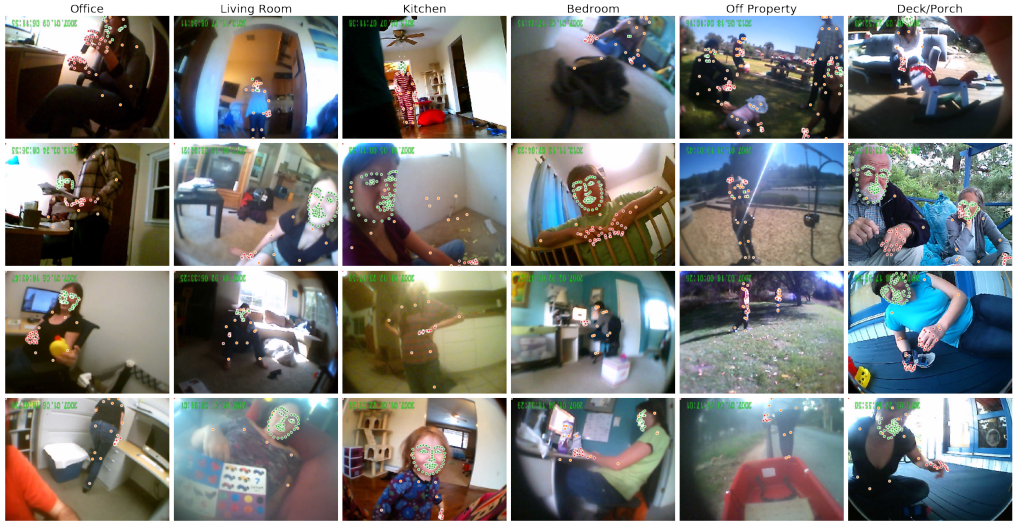
\includegraphics{figs/examples-1} 

}

\caption[Example frames taken from the dataset, illustrating variability in the infant perspective across different locations]{Example frames taken from the dataset, illustrating variability in the infant perspective across different locations. OpenPose detections are shown overlaid on these images.}\label{fig:examples}
\end{figure*}
\end{CodeChunk}

\subsection{Assessing automated social
annotations}\label{assessing-automated-social-annotations}

\subsubsection{Computer vision model}\label{computer-vision-model}

To automatically annotate the millions of frames in SAYcam, we use
OpenPose (Cao et al., 2018; Simon, Joo, Matthews, \& Sheikh, 2017). This
pose detector\footnote{\url{https://github.com/CMU-Perceptual-Computing-Lab/openpose}}
provided the locations of 18 body parts (ears, nose, wrists, etc.). The
system uses a convolutional neural network for initial anatomical
detection and subsequently applies part affinity fields for part
association, producing a series of body part candidates. The candidates
are then matched to a single individual and finally assembled into a
pose. Thus, while we only make use of the outputs of the face and hand
detections, the entire set of pose information from an individual is
used to determine the presence of a face/hand, making the process much
more robust to occlusion than methods optimized to detect only faces or
hands. Specifically, we tagged frames with detected nose keypoints as
having a face, and frames with a wrist keypoint were tagged as having a
hand.

\subsubsection{Manual annotation
strategy}\label{manual-annotation-strategy}

To test the validity of OpenPose's hand and face detections, we compared
the accuracy of these detections relative to human annotations of 24,000
frames selected uniformly at random from videos of two children (S and
A). Frames were jointly annotated for the presence of faces and hands. A
second set of coders recruited via AMT (Amazon Mechanical Turk)
additionally annotated 3150 frames; agreement with the primary coder was
\textgreater{}95\%.

\subsubsection{Detection accuracy for faces and
hands}\label{detection-accuracy-for-faces-and-hands}

As has been observed in other studies on automated annotation of headcam
data (e.g. {\textbf{???}}, ({\textbf{???}})), detection tasks that are
easy in third-person video can be quite challenging in egocentric
videos, due to difficult angles and sizes as well as substantial
occlusion. For example, the infant perspective often contains
non-canonical viewpoints of faces (e.g., looking up at a caregiver's
chin) as well as partially-occluded or oblique viewpoints of both faces
and hands.

To evaluate OpenPose's performance, we compared its detections to the
manually-annotated gold set of frames, calculating precision (hits /
hits + false alarms), recall (hits / hits + misses), and f-score (the
harmonic mean of precision and recall). In our data, for faces, the
F-score was 0.64, with a precision of 0.7 and recall of 0.58. For hands,
the F-score was 0.51, with a precision of 0.73 and recall of 0.4. While
face and hand detections showed moderately good precision, face
detections were overall slightly more accurate than hand detections.
Hand detections suffered from fairly low recall, indicating that
OpenPose likely underestimated the proportion of hands in the dataset.
We suspect that this is in part because children's own hands were often
in view of the camera and unconnected to a pose; this factor is explored
in detail in the following analysis section.

We also examined whether the precision, recall, and F-score for hands
and faces varied per child as a function of age to see if there was any
bias in the OpenPose detections related to age, and did not find
substantial variation. Nonetheless, while OpenPose was trained on
photographs from the adult perspective, this model still generalized
relatively well to the egocentric infant viewpoint with no fine-tuning
or post-processing of the detections.

\subsection{Access to social
information}\label{access-to-social-information}

\subsubsection{Changes across age}\label{changes-across-age}

We analyzed the social information in view across the entire dataset,
looking specifically at the proportions of faces and hands that were in
view for each child. Data from videos were binned according to the age
of the child (in weeks) (see Figure 2). First, when examining the
younger age ranges (\textless{} 24 months) we saw that the proportion of
faces in view showed a moderate decrease across this age range, both
when analyzing the random 24K frames as well as the entire dataset (see
Figure 2A).

While these trends appear somewhat different than those observed in
Fausey et al. (2016), note that Fausey et al. (2016) included data from
very young infants (from 1-4 months of age), while here the youngest
videos coming from S and A around 6 and 9 months of age, respectively.
Similarly, our age range extends 8 months later than those infants in
Fausey et al. (2016), throughout a portion of third year of life.

\begin{CodeChunk}
\begin{figure*}[h]

{\centering 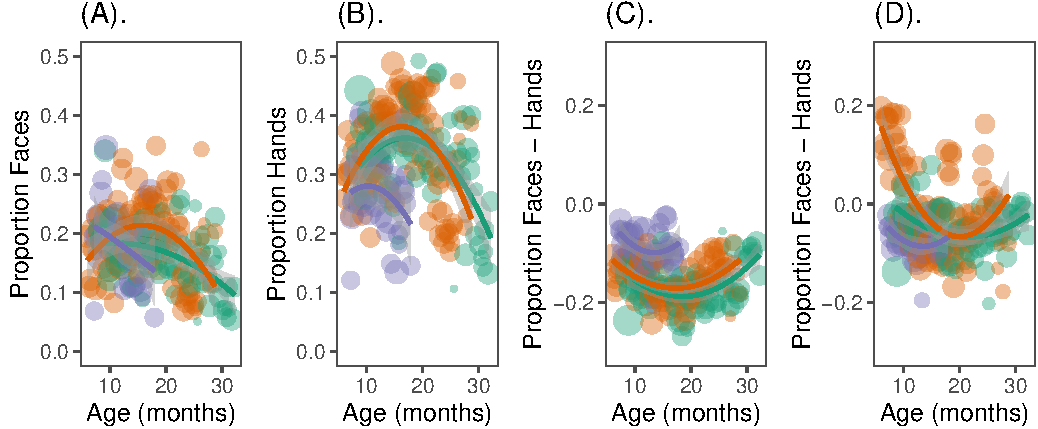
\includegraphics{figs/FaceVsHands-1} 

}

\caption[Proportion of faces vs]{Proportion of faces vs. hands in the entire dataset (A) and when hand detections are restricted to the upper 60 percent of the field of view (B). Data from each child (A, S) are plotted separately and binned by each week that the videos were filmed; data is scaled by the number of frames in that age range.}\label{fig:FaceVsHands}
\end{figure*}
\end{CodeChunk}

However, the most striking result is a much greater proportion of hands
in view than have previously been reported (Fausey et al., 2016). We
found this to be true across all ages, in both children, and regardless
of whether we analyzed human annotations (on the 24K random subset) or
OpenPose annotations on entire dataset. This is notable especially given
that OpenPose showed relatively low recall for hands, indicating that
this is still an underestimate of the proportion of hands in view. One
reason this could be the case is the much larger field of view that was
captured by the cameras used in this study: unlike previous studies, our
cameras were outfitted with a fish-eye lens in an attempt to capture as
much of the children's field of view as possible. Thus, the field of
view (FOV) of the fisheye lens used was larger (109 degrees horizontal x
70 degrees vertical) than the FOV of the lens used in many previous
studies; for example, in Fausey et al. (2016) the FOV was 69 x 41
degrees. This larger field of view may have allowed the SAYcam cameras
to capture not only the presence of a social partner's hands interacting
with objects, but also the children's own hands, leading to more
frequent hand detections.

\begin{CodeChunk}
\begin{figure}[h]

{\centering 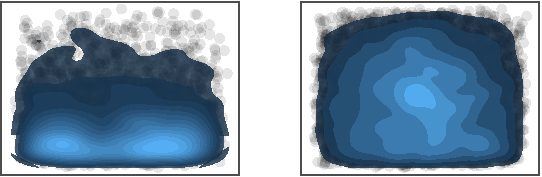
\includegraphics{figs/density-1} 

}

\caption[Density estimates for the child (left) and adult (right) hands that were detected int eh 24K random gold set]{Density estimates for the child (left) and adult (right) hands that were detected int eh 24K random gold set; each dot represents the center of a bounding box made by an adult participant.}\label{fig:density}
\end{figure}
\end{CodeChunk}

To assess this possibility, we obtained human annotations for a
subsample of 9051 frames in which a hand was detected in the random gold
set; participants (recruited via AMT) were asked to draw bounding boxes
around children's hands and adult's hands. Overall, we found that 34\%
of the hands in the random 24K sample were of children's own hands
(compared to 8\% reported in Fausey et al. (2016)) suggesting that this
difference in field of view did contribute substantially to the higher
rate of hand detections in the frames. Heatmaps of the bounding boxes
obtained from these annotations can be seen in Figure 3, showing that
children's hands tended to appear in the lower half of the frames.

We thus re-analyzed the entire dataset while restricting our analysis to
a smaller, upper portion of the frame comparable to the field of view
used in Fausey et al. (2016). To do so, we excluded hand detections that
occurred in the bottom 40\% of the frame, while retaining all hand
detections that occurred in the top 60\% of the frame. This coarse
cropping of decreased the proportion of hand detections from
0.3263743percent to 0.2156618 percent.

With this modified field of view, we now observed a more substantive
decrease across age in the proportions of faces relative to hands. To
quantify this trend, we fit a generalized linear mixed model to the
binned detection rates from this smaller field of field to estimate
changes in the proportion of faces vs.~hands over age. To better
approximate Fausey et al. (2016), we also restricted our analysis to the
age range seen in Fausey et al. (2016), excluding videos when children
were over 24 months of age, and indeed found that the proportion of
faces vs.~hands declined modestly with age (see Table 1).

However, when we considered the entire age range, we also observed an
unexpected trend in which the relative proportion of faces vs.~hands
increased again after 24 months of life; this trend was stronger in the
full dataset. While we did not have any a priori hypotheses about this
age range, we suspect that this could have to do with an increase in
children's independence from their caregiver as they master walking
around and interacting with objects in the world on their own.

\subsubsection{Variability by Location}\label{variability-by-location}

How does variability across different contexts influence the social
information in the infant view? Intuitively, some activities in
different contexts may be characterized by a much higher proportion of
faces (e.g., diaper changes in bedrooms) than others (e.g., playtime in
the living room). We thus next examined variation in presence of hands
and faces across different locations. Of the 1622 videos, 639 were
annotated (Sullivan et al., under review) for the location o videos were
filmed in. 296 were filmed in single location, representing 17 percent
of the dataset and over 5 million frames (see Sullivan et al. (under
review)). Activities varied somewhat predictability by these contexts:
for example, eating tended to occur in the kitchen, whereas playtime was
the dominant activity in the living room. Overall, we found that the
proportion of faces vs.~hands varied across filming locations, and, to
some extent, across children. For example, while both A and S saw a
relatively similar proportion of faces vs.~hands in the bedroom, they
saw quite different amounts of faces vs.~hands in kitchen.

\begin{CodeChunk}
\begin{figure}[h]

{\centering 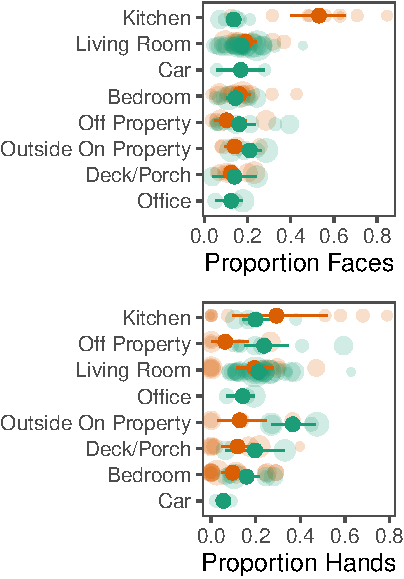
\includegraphics{figs/DetByLocation-1} 

}

\caption[Proportion of faces (A),  hands (B), and faces vs]{Proportion of faces (A),  hands (B), and faces vs. hands  (C) by location in which egocentric videos were filmed; data from individual children are plotted separately (location annotations were not available for Y). Data are only taken from the top 60 percent of the frames so as to minimize the contribution of children’s own hands. Each dot represents data from a week in which videos were filmed and are scaled by the number of frames (i.e., amount of video) in that datapoint.}\label{fig:DetByLocation}
\end{figure}
\end{CodeChunk}

\section{General Discussion}\label{general-discussion}

Broadly, the present analysis of this dense, longitudinal dataset has
yielded a better understanding of infants' evolving access to social
information. First, we found a relatively high proportion of faces in
view in the videos from the youngest age ranges in each child,
confirming previous findings (Fausey et al., 2016). This is particularly
notable given that, in cross-sectional data, this effect seems to be
most strongly driven by infants younger than 4 months of age (e.g.,
Fausey 2016; Jayaraman, Fausey, \& Smith, 2015; Sugden, Mohamed-Ali, \&
Moulson, 2014) who see both more frequent and more persistent faces
(Jayaraman \& Smith, 2018).

Second, we found considerable variability in the social information in
view depending on the activity context in which children were present.
Even within a given, well-defined context---mealtime---we found
variability across individual children. Intuitively, there are at least
three ways to feed a young child in a kitchen (i.e., forward facing the
child in a high chair, holding the child outward, or sitting side by
side with them) and these regularities in a child's life may hold a
larger influence over the amount of social information in view than
previously considered.

Finally, we demonstrate the feasibility of using a modern, off-the-shelf
computer vision model to vastly increase the efficiency of processing
egocentric headcam footage, allowing us to annotate the entirety of very
large datasets (here, \textgreater{}30 million frames) for the presence
and size of people, hands, and faces, representing a 300-fold increase
in data relative to prior work (Fausey et al., 2016). As these
detections were imperfect compared to human annotators, fine-tuning
these models to better optimize for the infant viewpoint remains an open
avenue for future work. Standard computer vision models are rarely
exposed on these naturalistic, egocentric viewpoints, and we suspect
that training these models on more naturalistic data may lead to more
robust, generalizable detectors.

These analyses have highlighted the importance of considering the
infants field-of-view when analyzing egocentric videos. In many frames
children's own hands were likely visible, due to the wide field of
view---capturing valuable information about what these children were
interacting with in different contexts across the first few years of
their life. Furthermore, though this choice more closely approximates
children's actual perspective, these viewpoints are still a proxy as we
do not know where in the frames children are allocating their attention.

Indeed, the questions of how, when, from whom, and what data we sample
become critically important when we attempt to construct naturalistic
datasets, and we would be remiss if we did not acknowledge the
limitations of the present dataset. While these data are longitudinal,
they are only sampled from representative of few children, all growing
up in relatively privileged households in western societies. Any
idiosyncrasies in how and when these particular families chose to film
these videos undoubtedly influences the variability seen here.
Nonetheless, we believe that these advances in methodologies and
datasets are a step in the right direction. The large-scale analysis of
dense datasets---collected with different fields of view, cameras and
from many different laboratories---has the potential to create
generalizable conclusions about the regularities of infant experience
that scaffold learning.

\section{Acknowledgements}\label{acknowledgements}

We would like to thank X and Y for helpful comments, and\ldots{}

\section{References}\label{references}

\setlength{\parindent}{-0.1in} \setlength{\leftskip}{0.125in} \noindent

\hypertarget{refs}{}
\hypertarget{ref-Cao2018openpose}{}
Cao, Z., Hidalgo, G., Simon, T., Wei, S.-E., \& Sheikh, Y. (2018).
OpenPose: Realtime multi-person 2D pose estimation using Part Affinity
Fields. In \emph{ArXiv preprint arXiv:1812.08008}.

\hypertarget{ref-Farroni2002}{}
Farroni, T., Csibra, G., Simion, F., \& Johnson, M. H. (2002). Eye
contact detection in humans from birth. \emph{Proceedings of the
National Academy of Sciences}, \emph{99}(14), 9602--9605.

\hypertarget{ref-Fausey2016}{}
Fausey, C. M., Jayaraman, S., \& Smith, L. B. (2016). From faces to
hands: Changing visual input in the first two years. \emph{Cognition},
\emph{152}, 101--107.

\hypertarget{ref-Gredeback2010}{}
Gredeback, G., Fikke, L., \& Melinder, A. (2010). The development of
joint visual attention: A longitudinal study of gaze following during
interactions with mothers and strangers. \emph{Developmental Science},
\emph{13}(6), 839--848.

\hypertarget{ref-Jayaraman2018}{}
Jayaraman, S., \& Smith, L. B. (2018). Faces in early visual
environments are persistent not just frequent. \emph{Vision Research}.

\hypertarget{ref-Jayaraman2015}{}
Jayaraman, S., Fausey, C. M., \& Smith, L. B. (2015). The faces in
infant-perspective scenes change over the first year of life. \emph{PLoS
One}. \url{http://doi.org/10.1371/journal.pone.0123780}

\hypertarget{ref-Sanchez2018}{}
Sanchez, A., Long, B., Kraus, A. M., \& Frank, M. C. (2018). Postural
developments modulate children's visual access to social information. In
\emph{Proceedings of the 40th annual conference of the cognitive science
society}.

\hypertarget{ref-Simon2017hand}{}
Simon, T., Joo, H., Matthews, I., \& Sheikh, Y. (2017). Hand keypoint
detection in single images using multiview bootstrapping. In
\emph{CVPR}.

\hypertarget{ref-Sugden2014}{}
Sugden, N. A., Mohamed-Ali, M. I., \& Moulson, M. C. (n.d.). I spy with
my little eye: Typical, daily exposure to faces documented from a
first-person infant perspective. \emph{Developmental Psychobiology},
\emph{56}(2), 249--261.

\hypertarget{ref-SAYcam}{}
Sullivan, J., Mei, M., Perfors, A., Wojcik, E., \& Frank, M. (under
review). Head cameras on children aged 6 months through 31 months.

\bibliographystyle{apacite}


\end{document}
